% Desargues: triangles ABC and A'B'C' in perspective from O; the side intersections P, Q, R are collinear.
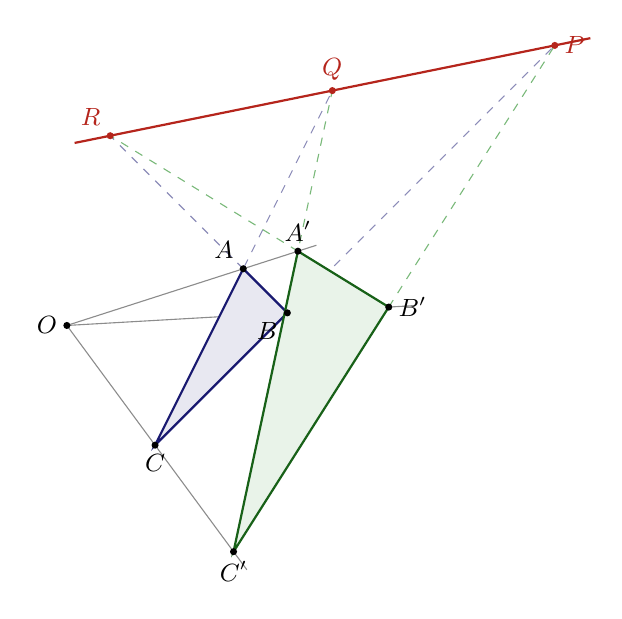
\begin{tikzpicture}[scale=0.8,font=\small]
\draw[black!45] (0.0000,0.0000) -- (3.9614,1.2733);
\draw[black!45] (0.0000,0.0000) -- (5.5188,0.3154);
\draw[black!45] (0.0000,0.0000) -- (2.8577,-3.8783);
\draw[MidnightBlue!50,dashed] (2.8000,0.9000) -- (0.6879,3.0121);
\draw[MidnightBlue!50,dashed] (3.5000,0.2000) -- (7.7459,4.4459);
\draw[MidnightBlue!50,dashed] (1.4000,-1.9000) -- (4.2142,3.7285);
\draw[ForestGreen!60,dashed] (3.6680,1.1790) -- (0.6879,3.0121);
\draw[ForestGreen!60,dashed] (5.1100,0.2920) -- (7.7459,4.4459);
\draw[ForestGreen!60,dashed] (2.6460,-3.5910) -- (4.2142,3.7285);
\draw[MidnightBlue,thick,fill=MidnightBlue!10] (2.8000,0.9000) -- (3.5000,0.2000) -- (1.4000,-1.9000) -- cycle;
\draw[ForestGreen!70!black,thick,fill=ForestGreen!10] (3.6680,1.1790) -- (5.1100,0.2920) -- (2.6460,-3.5910) -- cycle;
\draw[BrickRed,thick] (0.1232,2.8974) -- (8.3106,4.5606);
\fill[black] (0.0000,0.0000) circle (1.6pt) node[left,black] {$O$};
\fill[black] (2.8000,0.9000) circle (1.6pt) node[above left,black] {$A$};
\fill[black] (3.5000,0.2000) circle (1.6pt) node[below left,black] {$B$};
\fill[black] (1.4000,-1.9000) circle (1.6pt) node[below,black] {$C$};
\fill[black] (3.6680,1.1790) circle (1.6pt) node[above,black] {$A'$};
\fill[black] (5.1100,0.2920) circle (1.6pt) node[right,black] {$B'$};
\fill[black] (2.6460,-3.5910) circle (1.6pt) node[below,black] {$C'$};
\fill[BrickRed] (7.7459,4.4459) circle (1.6pt) node[right,BrickRed] {$P$};
\fill[BrickRed] (4.2142,3.7285) circle (1.6pt) node[above,BrickRed] {$Q$};
\fill[BrickRed] (0.6879,3.0121) circle (1.6pt) node[above left,BrickRed] {$R$};
\end{tikzpicture}
